\chapter{Simulation}
	We provided the initial output in a web interface. The following figure shows the first appearance of our simulation environment when we access to the local server. \\
	
	\begin{figure}[H]
		\centering
		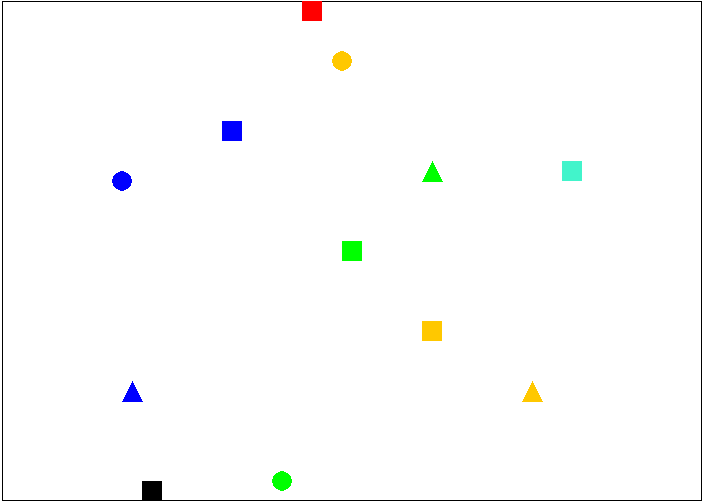
\includegraphics[scale=0.35]{environment}
		\caption{First Appearance of the Environment}
	\end{figure}
	\vline
	
	The instruction we give in voice not all are properly detected by our used speech recognition module. In this simulation we modified the detected text here.\\
	
	If we give voice instruction: `Go from Cruzon Hall to TSC through Shaheed Minar', the output in the environment will look like as follow. \\
	\begin{figure}[H]
        \centering
        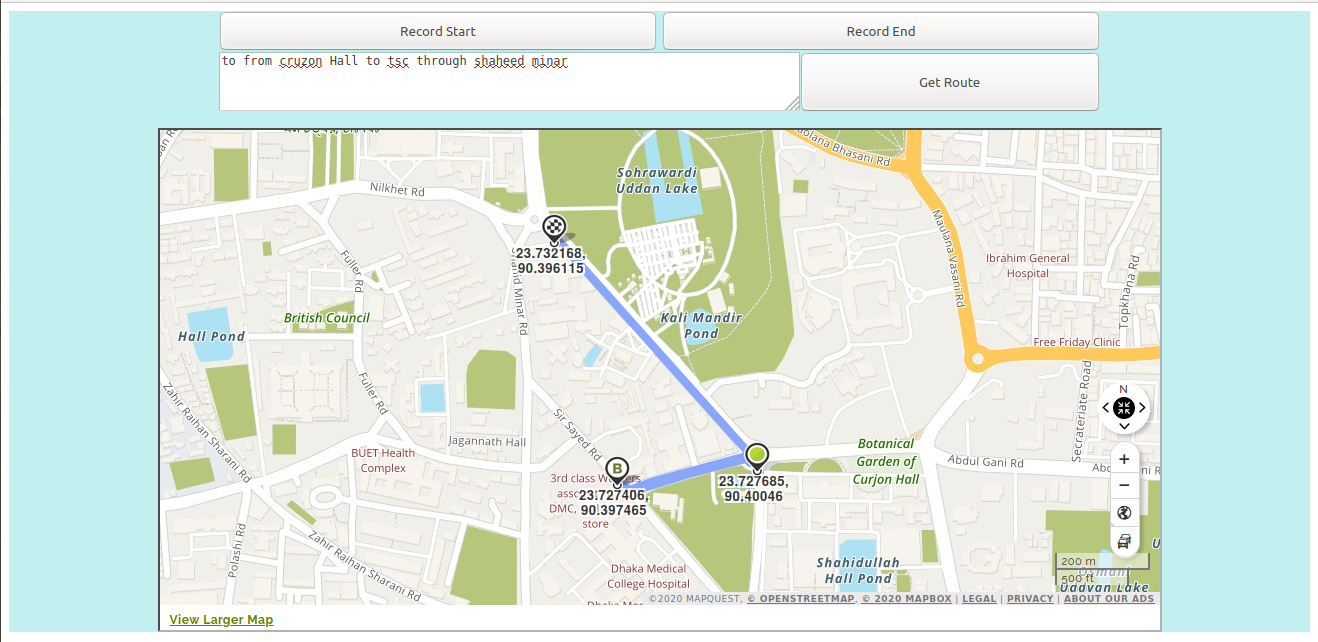
\includegraphics[scale=0.30]{simulation1}
        \caption{Output for an Instruction}
    \end{figure}
    \vline
	
	As the models sometimes makes error, here is a erroneous case. For instruction `Go from Bangla Academy to Dhaka Medical college through Shahidullah Hall', the model detected Dhaka Medical College as source instead of destination and similarly detect Bangla Academy as destination instead of source. \\
	\begin{figure}[H]
        \centering
        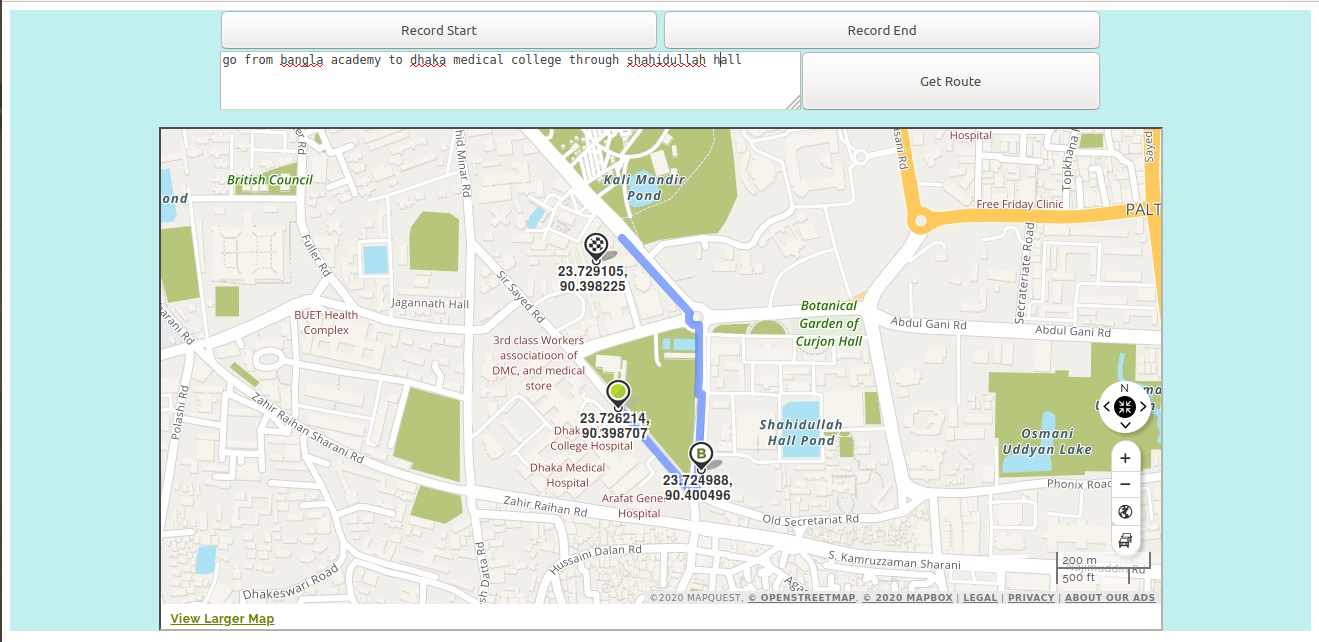
\includegraphics[scale=0.30]{simulation2}
        \caption{A Wrong Output for Another Instruction}
    \end{figure}
    \vline
	
	\textbf{Hardware} \\
	We also have designed a simple line following robot which is able to follow the instruction we gave in voice. We make a dummy track where the robot assumes some node as some real location. The following figure shows our designed line following robot.
	\begin{figure}[H]
		\centering
		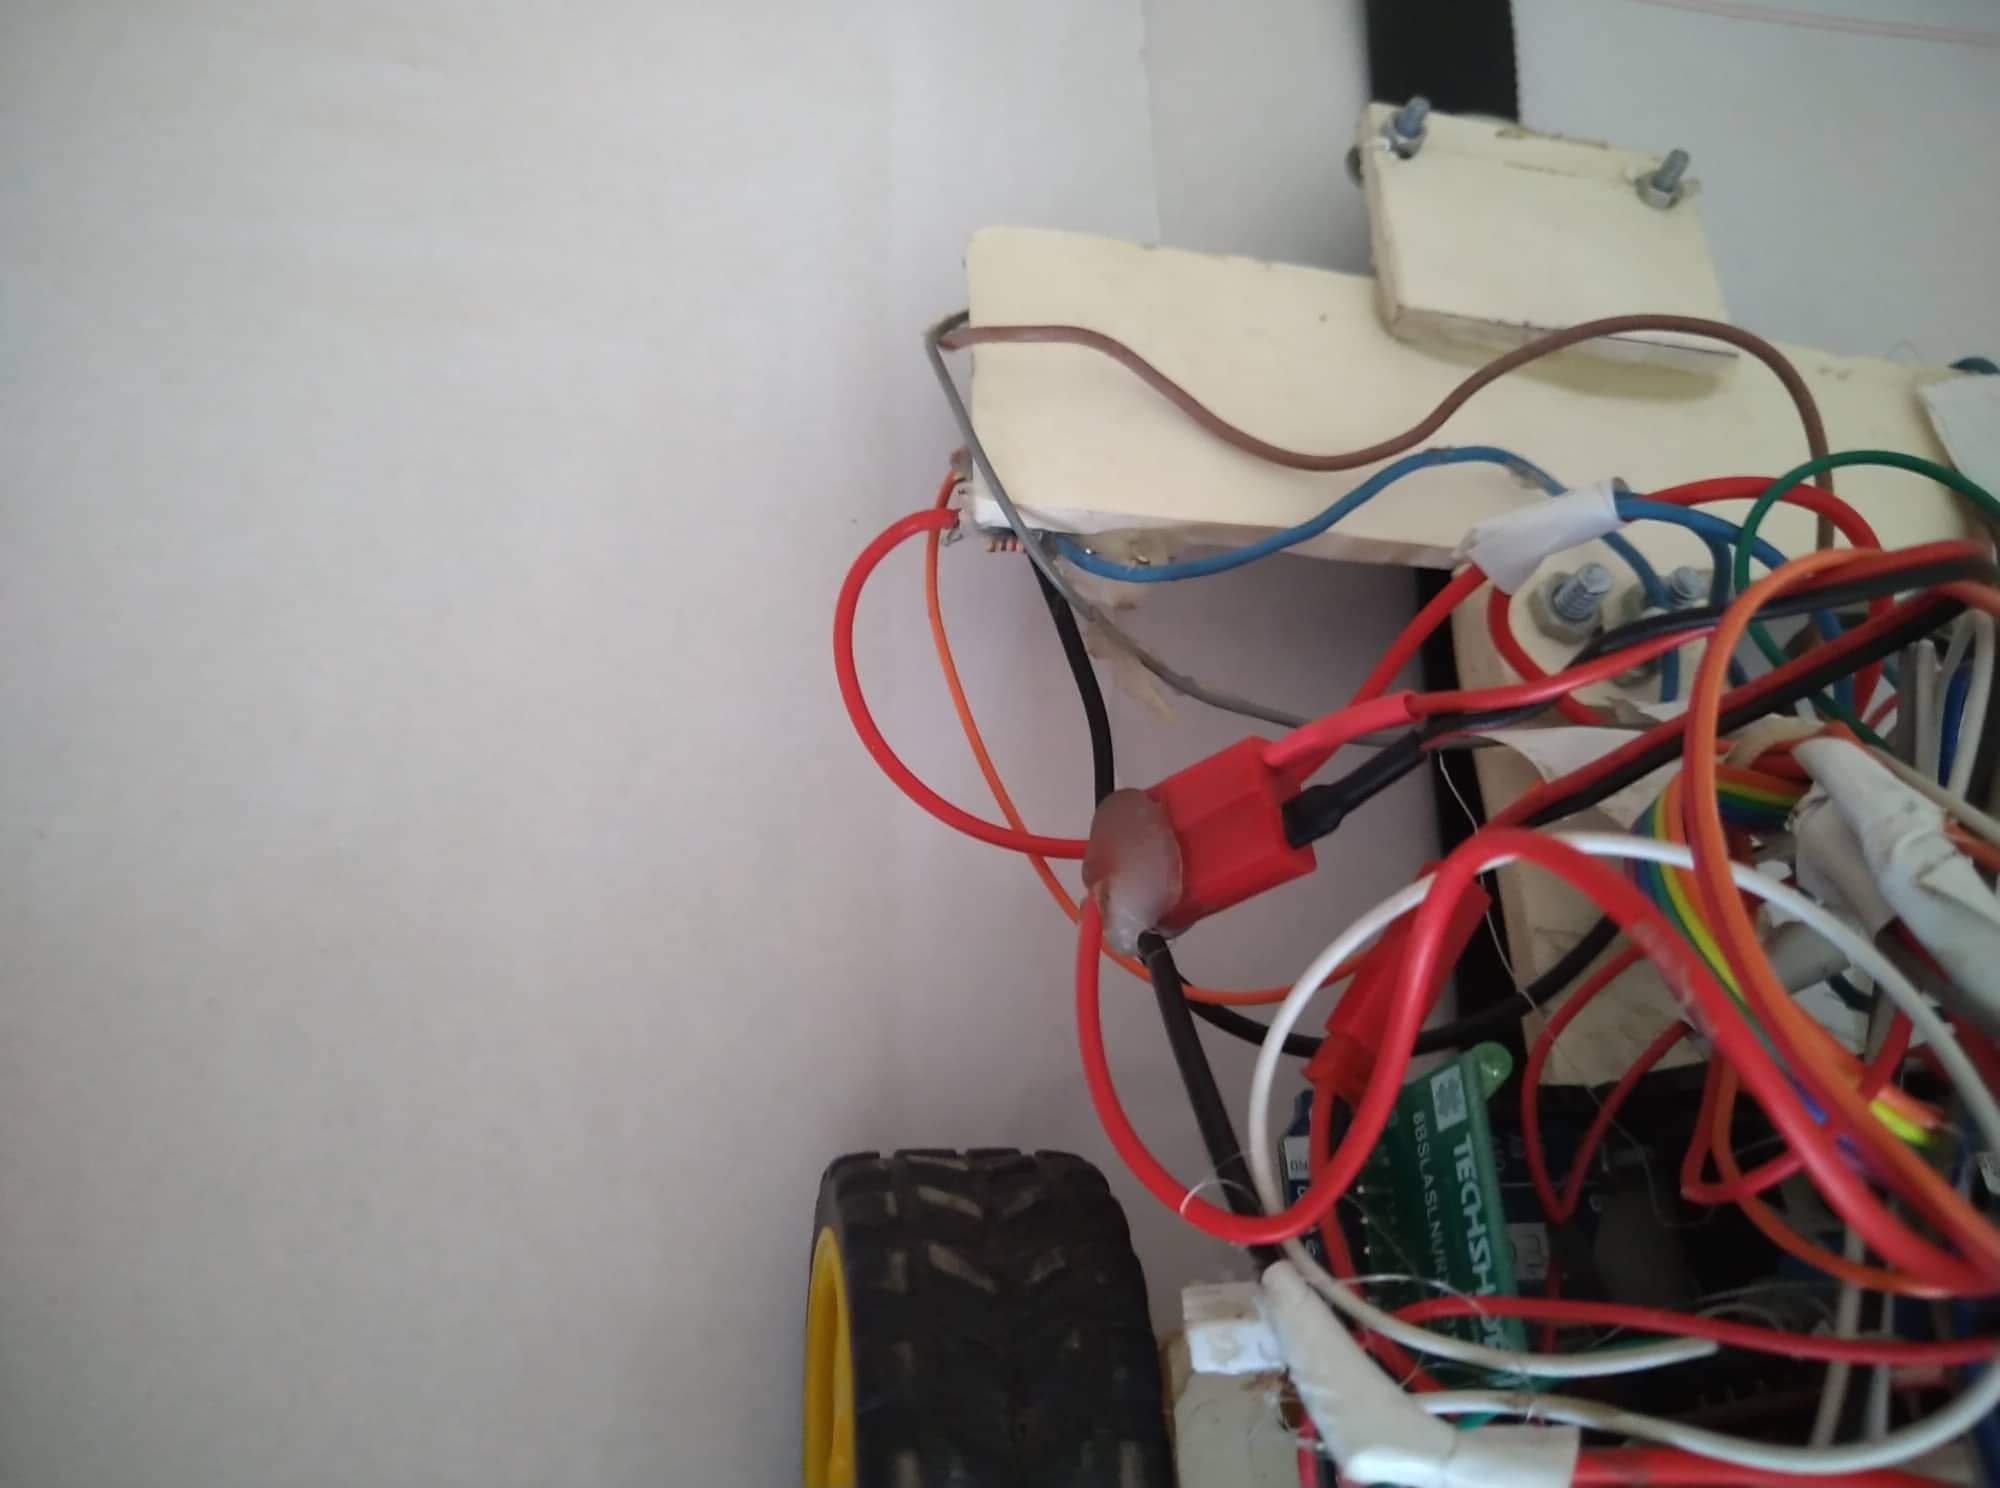
\includegraphics[scale=0.20]{line_follower}
		\caption{A Simple Line Follower for Simulation}
	\end{figure}
	\vline